\documentclass[12pt,a4paper]{article}

% ==== PACKAGES (ordered, no duplicates) ====
\usepackage[T1]{fontenc}
\usepackage[utf8]{inputenc}
\usepackage[english]{babel}
\usepackage{lmodern}
\usepackage{geometry}
\geometry{margin=1in}
\usepackage{setspace}
\onehalfspacing
% PREÁMBULO
\usepackage{pdfpages}
\usepackage{caption}    % para usar \captionof
\usepackage{graphicx}
\usepackage{float}
\usepackage{subcaption}
\usepackage{booktabs}
\usepackage{longtable}
\usepackage{xcolor}
\usepackage{listings}
\usepackage{enumitem}
\usepackage{titling}


% ==== HYPERREF LAST ====
\usepackage{hyperref}
\hypersetup{
  colorlinks=true,
  linkcolor=blue,
  citecolor=blue,
  urlcolor=blue
}

% ==== HELPERS ====
\newcommand{\todo}[1]{\textcolor{red}{[TODO: #1]}}

% Custom subtitle using titling
\pretitle{\begin{center}\Large\bfseries}
	\posttitle{\par\vspace{0.5em}\large\itshape First Report\end{center}\vspace{1em}}


% ==== TITLE ====
\title{\textbf{Design and Implementation of a Web System for Searching and Managing Courses - Course Finder}}

\author{%
  Brayan Alejandro Riveros Rodríguez \and
  Cristian Santiago Ríos Vásquez \and
  Carlos Andres Pescador Castro\\[0.25em]
  \normalsize Systems Engineering\\
  \normalsize Universidad Distrital Francisco José de Caldas
}
\date{\today}

\begin{document}
	
\maketitle

\begin{abstract}
Students often must search through numerous of courses, multiple instructors, and changing schedules across semesters, but information is often not centralized or in a palatable format, or in partially synchronized systems, making discovery and planning difficult. This project proposes a web-based system that consolidates course data and formalizes instructor-course relationships, separating authentication/authorization services from central domain-based course services, with non-functional objectives to integrate and centralize data, efficient search, and course-instructor associations. Workshops 1 and 2 established the central problem using business model canvas, user stories, CRC cards, and overall system design. Guided by Scrum as a development management methodology, preparing for sprint planning and traceability, this first report summarizes preliminary results and describes the project road map.
\end{abstract}

\tableofcontents
\listoffigures
\listoftables
\newpage

% ======================================================================
\section{Introduction}
\label{sec:intro}

\subsection{Context and Motivation}
Students often have no way to organize their semester schedules. At many institutions, including our own, course information is often poorly organized. This fragmentation makes it difficult for students to discover relevant offerings of interest, as well as the professors who teach them and their schedules. The result is avoidable problems during planning and registration periods, duplicate registrations, and delays in decision-making.\newline

To address these issues, we propose a web system for searching and managing academic courses that consolidates essential data (course codes, titles, descriptions) and formalizes the relationships between professors and courses. The system targets three primary stakeholder groups: (i) \textit{students}, who need fast, accurate search and discovery; (ii) \textit{professors}, who is the associated with the courses; and (iii) \textit{administrators users}, which is responsible for loading the data and managing the application. Our current work established the problem framing and initial design assets for the development phase.\newline

From an engineering perspective, the project is intentionally designed to practice delivering end-to-end software within a semiannual schedule by implementing an agile approach.

\subsection{Objectives}
\begin{itemize}[leftmargin=1.2em]
  \item Design and specify a reliable web-based system that allows key stakeholders to search, manage and maintain accurate information about courses and instructors.
  \item Define a clear and feasible road map for the implementation of the project that aligns with the identified problem context, stakeholder needs, and planning.
  \item Synthesize the context, stakeholders, and scope of the problem into a consistent baseline that unifies terminology and guides subsequent design and development activities.
\end{itemize}


\subsection{Scope}
This first report defines the requirements and design boundaries of the project at its current stage. It focuses on consolidating the conceptual and architectural foundations, including problem definition, stakeholder identification, user stories, CRC cards, high-level architecture, deployment views, and early user-interface sketches. The report also introduces preliminary elements for the data model and API contracts that will guide the implementation in the next phase. This scope explicitly includes documenting the problem context, justifying the proposed solution, and establishing an initial road map under agile methodology using Taiga as the project management tool.


% ======================================================================
\section{Related Work and Background}
\label{sec:related}

 Students need digital systems to search and manage academic information such as course offerings, instructor assignments, and scheduling. However, on many occasions they find that in fragmented data or centralized in legacy applications that lack interoperability and transparency for stakeholders. In this context, academic management systems and course catalog platforms such as Moodle, Blackboard, and Google Classroom provide partial solutions, focusing primarily on learning management rather than the structural organization of academic offerings.\newline

From a technical point of view, modern web-based architectures rely on Restful API s, micro-service decomposition, and standard authentication mechanisms such as JWT (JSON Web Token) to ensure secure and maintainable information exchange. These principles underpin the design of this project: a lightweight, modular system divided into a authentication service and a business  This dual-back-end structure supports scalability, separation of concerns, and parallel development by different team members. Furthermore, adopting a continuous integration and deployment pipeline through tools like Docker and GitHub Actions allows the project to align with current DevOps practices that promote automation, repeatability, and early defect detection.\newline

In terms of methodology, the use of Scrum supported support on the Taiga tool reflects an agile approach, iterative development of software engineering. Agile methods are widely used in both industry and academia to encourage adaptability, transparency, and stakeholder feedback. Previous studies and projects in software engineering have shown that integrating agile practices allows for better quality deliveries.\newline

In summary, this work draws on principles from web-based academic management systems, requirement analysis and software design to propose a simple, fast, and verifiable solution tailored to the needs of the stakeholders.


% ======================================================================
\section{Methodology}
\label{sec:method}

\subsection{Process and Team Practices}
The project will follows an agile software development approach based on the Scrum framework, adapted to the context of problem. The team uses \textbf{Taiga} as the main project management tool to maintain the product backlog, define sprint goals, and track progress through user stories and tasks.\newline

Roles are distributed collaboratively among the three members of the team. Carlos Andres Pescador Castro serve as the Product Owner and is the responsible for prioritizing the backlog and maintaining alignment with the defined requirements. Cristian Santiago Ríos Vásquez act as the Scrum Master, facilitating coordination among team members, ensuring adherence to Scrum events, and managing sprint reviews and retrospectives. Brayan Alejandro Riveros Rodríguez as the Development Lead, focusing on technical implementation, version control integration, ci/cd pipeline and testing coordination. All members contribute equally to documentation, gathering of requirements and continuous improvement activities.\newline

Scrum ceremonies are conducted at a scaled frequency appropriate brief stand-up meetings are held twice per week (asynchronous when needed), sprint planning and retrospectives occur at the beginning and end of each workshop, and sprint reviews coincide with workshop submissions.\newline

Version control and collaboration are managed through a shared Git repository, following a feature-branch workflow. 


\subsection{System Analysis and Design}
Following the completion of Workshops~1 and~2, the system analysis and design phase guide the transition from requirements specification to technical implementation. The main goal will be to ensure that the proposed architecture, domain entities, and component responsibilities are consistent with the user stories, acceptance criteria, and stakeholder needs identified during the analysis stage.\newline

The analysis focus on consolidating the functional requirements derived from the user stories created in Workshop~1. Each user story will be mapped to a corresponding set of system components, defining clear inputs, processes, and outputs. CRC (Class–Responsibility–Collaborator) cards previously designed will serve as the foundation for assigning responsibilities among classes, while maintaining object-oriented design principles. This mapping will guarantee that each functional requirement has a direct representation within the software model.\newline

The system will adopt a modular architecture divided into two main backend services: an authentication and authorization service, and a core domain service for managing courses, professors, and their relationships. Both services will communicate through RESTful APIs, enabling independent deployment and scalability. Each backend will interact with its respective database—MySQL for authentication and PostgreSQL or MongoDB for the core domain—ensuring persistence and referential integrity across entities. The frontend web interface, developed with modern JavaScript framework, will consume these APIs to provide a cohesive user experience.\newline

To formalize the design, UML diagrams are used to illustrate the system structure and interactions. A class diagram will describe the main domain entities (Professor, Course, and Link), their attributes, and associations. A deployment diagram will detail how components will be distributed across environments, showing the web client, API services, and database instances.\newline

Non-functional requirements will also guide the design. The system will ensure security through JWT-based authentication and role-based access control, maintainability through modular coding practices, and performance through optimized database queries and API endpoints. Furthermore, logging and basic monitoring mechanisms will be defined to support future testing and evaluation.\newline

This analysis and design process will establish a clear technical blueprint for the implementation stage to be developed in Workshop~3. By grounding each architectural decision in the previously validated requirements, the team will ensure traceability from stakeholder needs to system components and a solid foundation for the subsequent development and testing phases.


% ======================================================================
\section{Implementation Progress (Workshops Summary)}
\label{sec:progress}
\subsection{Web UI}
This section presents the main artifacts developed during all the Workshops, which represent the foundation for the system implementation. Each artifact serves a specific purpose in documenting the design decisions and validating the feasibility of the proposed solution. The progression from conceptual models to concrete specifications ensures traceability from requirements to implementation.

\includepdf[
  pages=-,
  scale=0.9,
  pagecommand={%
    \thispagestyle{plain}%
    \centering
    \captionof{figure}{Web UI Mockup (v1.0)}
  }
]{"5. WebUI MockUps.pdf"}


The user interface was designed following the principle "Simple. Clear. Consistent." The visual design prioritizes clarity, usability, and role-based access control to ensure that each stakeholder group can efficiently accomplish their tasks without unnecessary complexity. Six main views were designed and subsequently implemented in the production environment, representing the complete user journey through the system.\newline

The interface accommodates three distinct user roles with different access levels and capabilities. Anonymous users can access the search functionality, allowing them to query courses by code, title, or professor details without authentication. The search results display comprehensive course information including schedules and associated instructors. Authenticated administrators access additional views for data management, including CRUD operations for courses and professors, as well as the assignment interface that links professors to specific courses and groups.\newline

Design decisions emphasized consistency across views through standardized navigation patterns, uniform typography, and coherent color schemes that distinguish between public and administrative sections. The responsive layout adapts to different screen sizes, ensuring accessibility across desktop and mobile devices. Form validation provides immediate feedback to users, reducing errors during data entry. The role-based design ensures that administrative functions remain hidden from unauthorized users while maintaining an intuitive experience for all stakeholder groups.\newline

The previous figures presents the final implemented views of the web application, demonstrating the translation from initial mockups to functional interfaces. These views validate the usability requirements established during the requirements analysis phase and confirm that the system meets the interaction needs identified in the user stories.


\subsection{Architecture Overview}
The system architecture implements a microservices approach with clear separation of concerns across three main components: frontend, an authentication service and a business logic service. This architectural decision was mandated by project requirements and offers several strategic advantages for development, deployment, and maintenance.\newline

The separation of authentication into an independent service provides security isolation, ensuring that credential management and token generation occur in a dedicated, hardened environment. This service connects to a database optimized for transaction processing and user session management. The authentication service issues JWT tokens upon successful login, which are subsequently validated by the business logic service for protected endpoints. This token-based approach enables stateless authentication, simplifying horizontal scaling and load balancing.\newline

The business logic service handles all domain operations including course management, professor administration, search functionality, and relationship assignments. By isolating these operations in a separate service connected to a database different from the one used for authentication, the system achieves better performance through database specialization.\newline

Component communication follows RESTful principles through well-defined API contracts. The frontend makes HTTPS requests to both backend services, with the authentication service providing tokens and the business service consuming them for authorization. This loose coupling allows independent deployment and version management of each service. Furthermore, the architecture supports parallel development, enabling team members to work simultaneously on different services without integration conflicts.\newline

\begin{figure}[H]
	\centering
	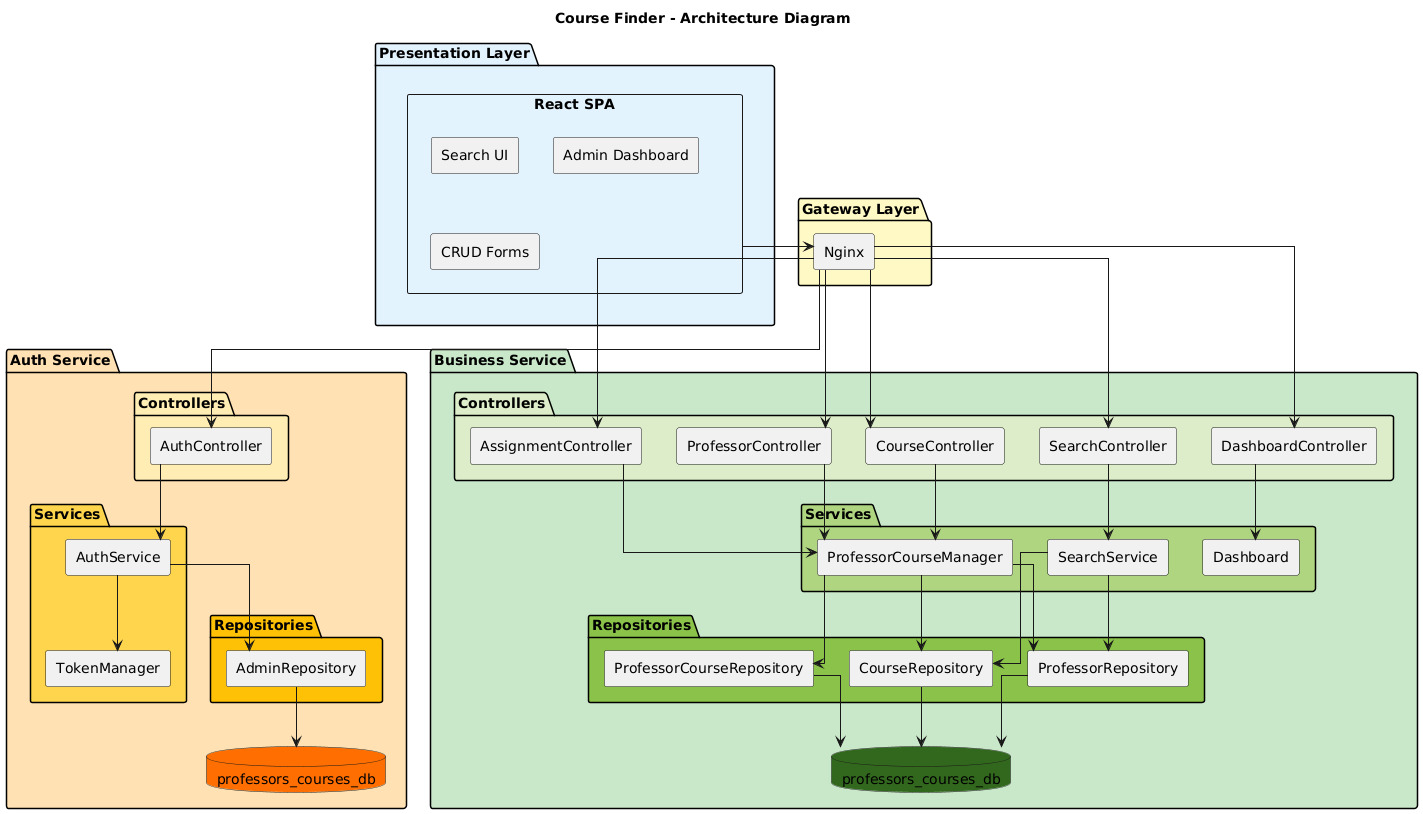
\includegraphics[width=0.9\linewidth]{diagramaArquitectura.png}
	\caption{Architecture Diagram (v1.0).}
	\label{fig:arch}
\end{figure}

Figure~\ref{fig:arch} illustrates the high-level architecture, showing the relationships between components, the data flow from user interaction through business logic to persistence layers, and the external interfaces exposed by each service. This diagram serves as the reference model for understanding system boundaries and component responsibilities throughout the development process.

\subsection{Deployment View}
\begin{figure}[H]
  \centering
  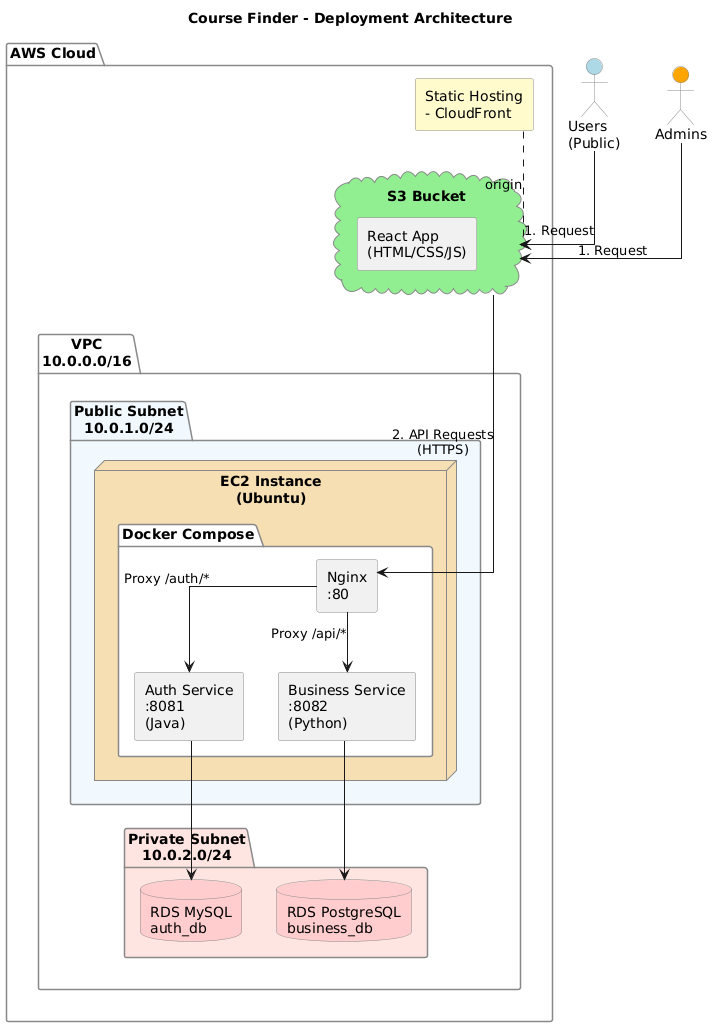
\includegraphics[width=0.9\linewidth]{deployDiagram.png}
  \caption{Deployment diagram (v1.0).}
  \label{fig:deploy}
\end{figure}

\subsection{Data Model}

The data model defines four primary entities that capture the essential academic domain: Professor, Course, Admin, and ProfessorCourse. This structure was designed to support the core user requirements identified during the analysis phase, particularly the need to search courses by multiple criteria and maintain clear associations between professors and their teaching assignments.\newline

The Professor entity contains identification attributes (id, username, name) and a specialty field that categorizes the instructor's academic area. This information enables filtering and grouping operations in search queries. The Course entity includes structural attributes (id, code, name) along with academic metadata (credits, category) that support both discovery and academic planning. The unique course code constraint ensures data integrity and prevents duplicate registrations.\newline

The relationship between professors and courses implements a many-to-many association through the ProfessorCourse junction entity. This design decision reflects the reality of academic scheduling where one professor may teach multiple courses and one course may be taught by multiple professors across different groups or semesters. The ProfessorCourse entity includes additional context such as groupId (to distinguish sections), assignedAt (for temporal tracking), and status (to manage active versus historical assignments). This rich association model provides the flexibility required for complex academic scenarios while maintaining referential integrity.\newline

The Admin entity remains separate from the academic domain, containing only authentication-relevant attributes (id, username, passwordHash, email). This separation ensures that administrative access control does not interfere with the core domain logic and allows for independent security policy management.\newline

Design decisions prioritized query performance for the primary use case: searching courses by professor or course attributes and retrieving all related information in minimal database operations. The normalized structure prevents data redundancy while the junction entity enables efficient joins. Repository interfaces abstract database operations, providing a clean separation between domain logic and persistence mechanisms that facilitates future database migration or optimization.\newline


\begin{figure}[H]
	\centering
	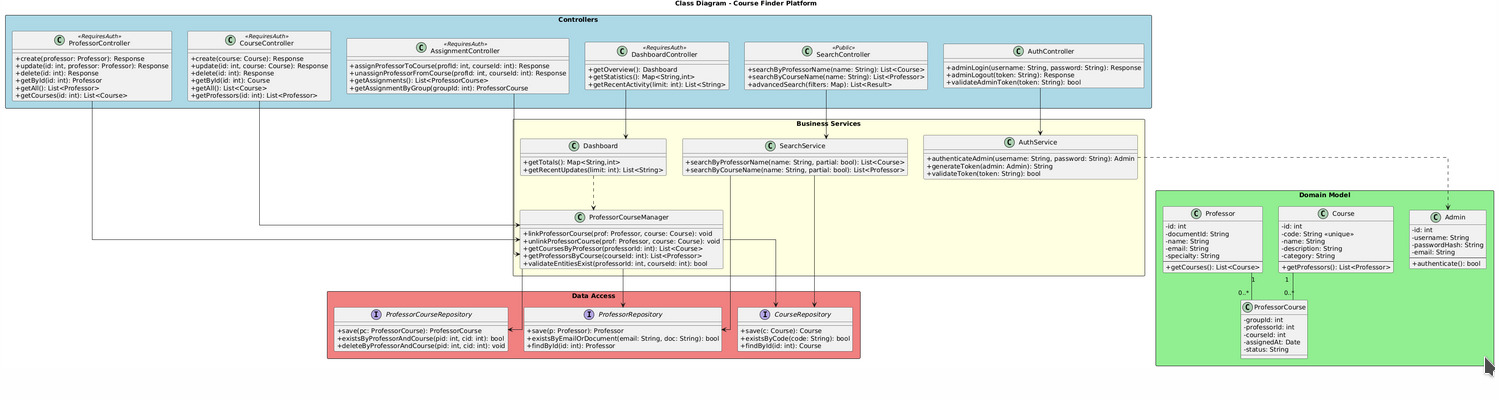
\includegraphics[width=0.9\linewidth]{diagramaClases.jpg}
	\caption{Class diagram (v1.0).}
	\label{fig:classdiagram}
\end{figure}

Figure~\ref{fig:classdiagram} presents the complete class diagram including entities, repositories, services, and controllers across all architectural layers. This diagram demonstrates how the data model integrates with business logic components and exposes functionality through controller endpoints. The layered structure visible in the diagram reinforces the architectural principles of separation of concerns and dependency management established in the system design.


% ======================================================================
\section{Results and Discussion}
The outcomes of Workshops~1 and~2 have established a solid analytical foundation for the project. The main deliverables include the problem definition, user stories with acceptance criteria, CRC cards, architectural and deployment diagrams, and early Web UI mockups. These artifacts provide a coherent view of the system’s objectives and structure, enabling the team to validate the feasibility of the proposed solution before implementation.


% ======================================================================
\section{Conclusions}
\label{sec:conclusions}
This first report consolidates the analytical and design foundations of the project, demonstrating coherent progress from requirement elicitation to system architecture definition. The established artifacts and planning ensure a clear path toward implementation, testing, and integration in the following workshop stages.


\section*{Glossary}
\begin{description}
  \item[API] Application Programming Interface.
  \item[CI/CD] Continuous Integration / Continuous Deployment.
  \item[JWT] JSON Web Token.
  \item[CRC] Class - Responsability - Collaboration Cards
\end{description}


\end{document}
